\chapter{PatchTST-Based Time-Series Classification}\label{ch:methodology}
%overview of the methodological pipeling
This chapter explains in Section \ref{sec:patchtst} how the PatchTST architecture works, how it is adapted for classification and what the selected hyperparameters are. Then follows in Section \ref{sec:train_eval} the training and evaluation procedure for PatchTST.

\section{PatchTST}\label{sec:patchtst}
PatchTST stands for Patch Time Series Transformer and is first introduced by Nie et al. in the paper called "\textit{A Time Series Is Worth 64 Words: Long-term Forecasting with Transformers}" \cite{nieTimeSeriesWorth2023b}. The researchers developed PatchTST for forecasting multivariate time series data, emphasizing channel-independence, for 8 different datasets, including weather data, traffic road occupancies from freeway sensors and hourly electricity consumption over time.

The core idea of the original PatchTST is to divide a multivariate time series into short patches and to use these patches as input tokens for a Transformer encoder. In the original formulation, patching and channel-independence are the two central design principles, where each sensor channel is processed as an individual univariate series, while the embedding layer and Transformer weights are shared across channels \cite{nieTimeSeriesWorth2023b}. In this way, PatchTST reduces the number of input tokens instead of tokenizing each time-step, thus being able to model longer contexts with lower quadratic attention cost.

For the insertion-classification task of this thesis, the general patch-based Transformer principle is kept, but the architecture is adapted in several important ways. First, the forecasting head of the original model is replaced by a classification head that outputs a single logit for binary success/failure classification. Second, the implemented model does not use the original channel-independent processing path, but a channel-mixing tokenization, in which all selected sensor channels of one patch are concatenated before tokenizing them.
The following \figref{fig:patchtst} shows the adapted architecture and how the data flows through the model. After the figure each step mentioned on the left side is explained in detail.
\begin{figure}[htpb]
    \centering
    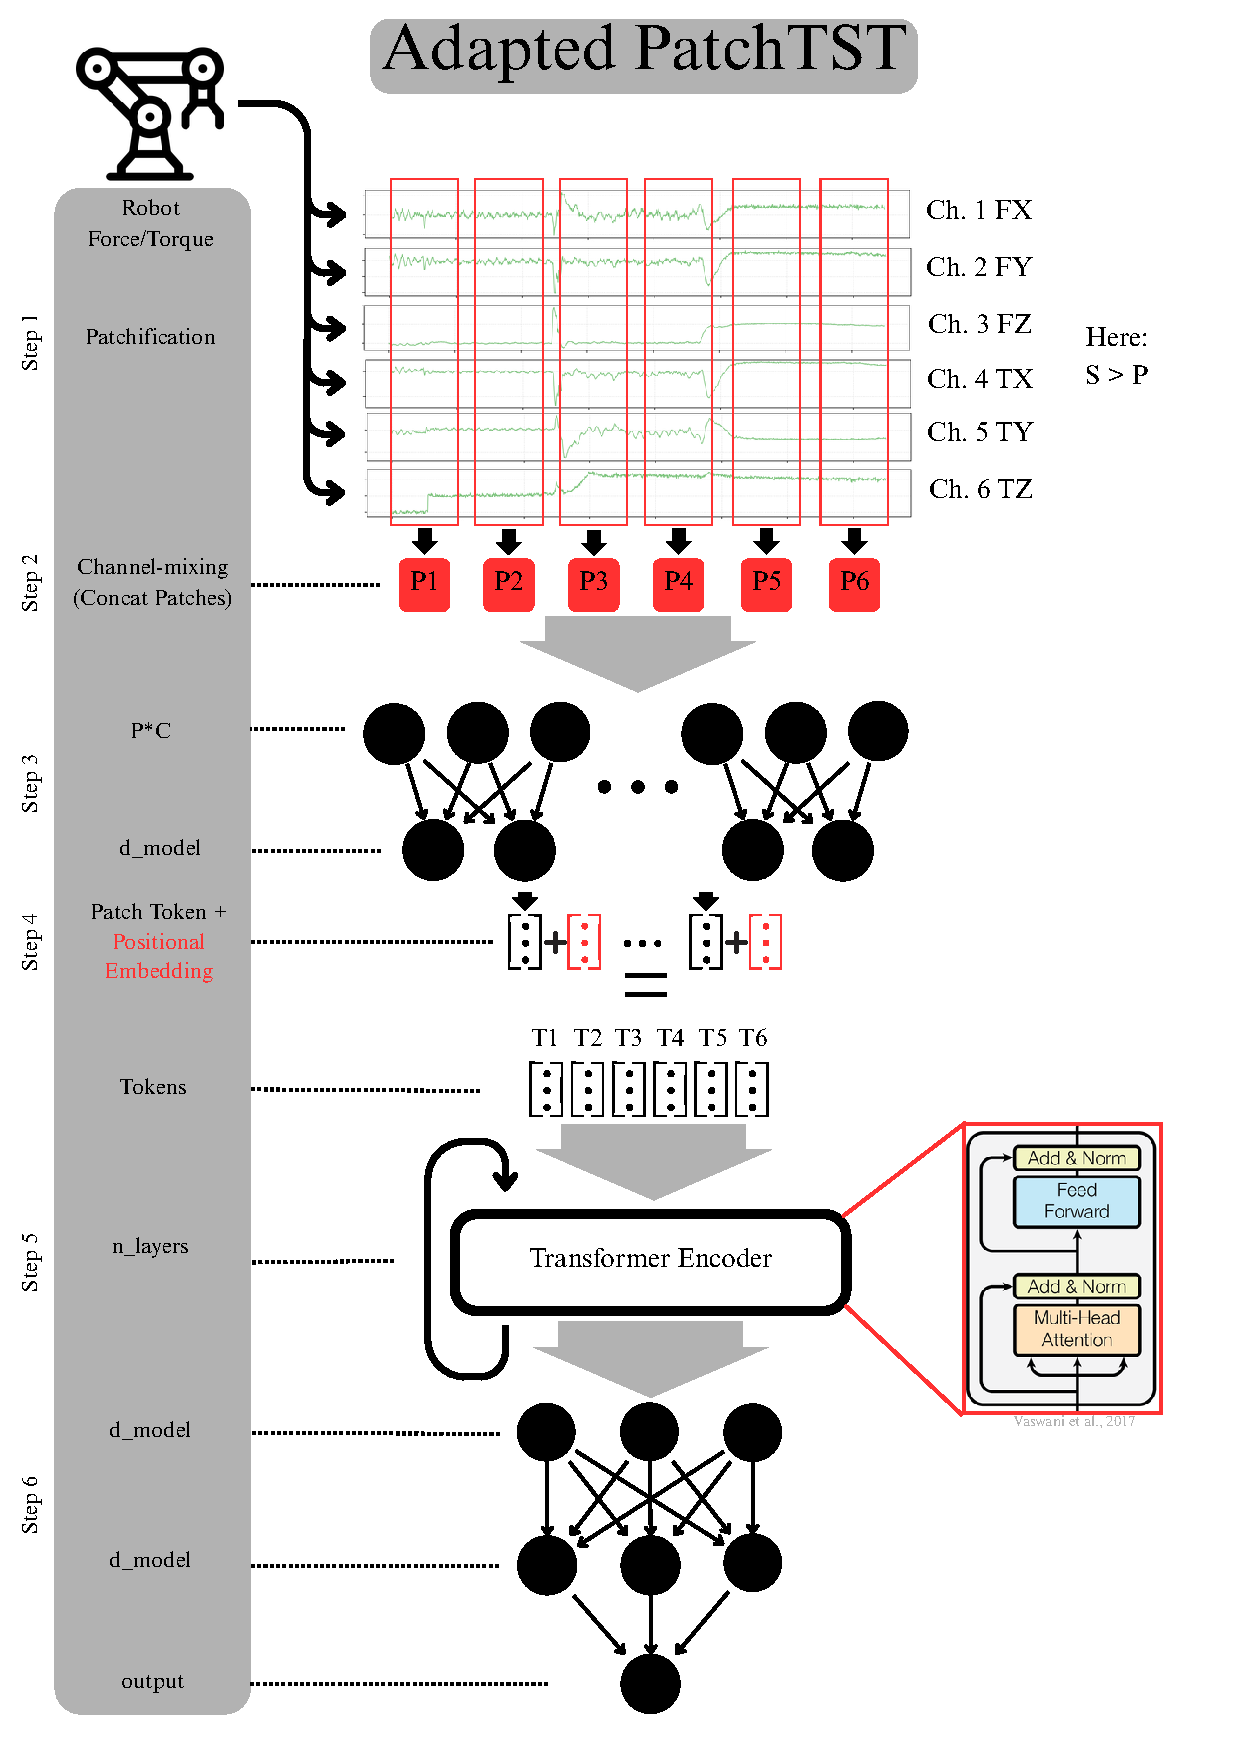
\includegraphics[width=0.95\textwidth]{chapters/5-patchtst/Patch extraction.pdf}
    \caption{Visual representation of the data flow in the adapted PatchTST architecture. The variables $P, C, S$ denote the patch length $P$, the number of used input channels $C$ and the stride step size $S$. Step 1: Patchification, Step 2: Channel-mixing, meaning concatenation of patches from all channels, Step 3: Tokenization/Projection of patches into patch tokens, Step 4: Final Tokens = Patch Token + Positional Embedding, Step 5: n\_layers of stacked Transformer Encoders, Step 6: Classification head.}
    \label{fig:patchtst}
\end{figure}
\newpage


Let one sequence be represented as a multivariate time series
\begin{equation}
\mathbf{X} \in \mathbb{R}^{L \times C},
\end{equation}
where $L$ denotes the sequence length and $C$ the number of selected input channels. In the implemented network, the batched input tensor is arranged as
\begin{equation}
\mathbf{X}_{\text{batch}} \in \mathbb{R}^{B \times L \times C},
\end{equation}
with batch size $B$. For the experiments in this thesis, the sequence length is fixed to $L=1500$, corresponding to a 3\,s recording at 500\,Hz.

\paragraph{Patch extraction, \figref{fig:patchtst} Step 1}
The first processing step is the patchification of the sequence. A patch length $P$ and stride $S$ are defined. Stride is the non overlapping region between two consecutive patches \cite{nieTimeSeriesWorth2023b}. In the implementation used here, $P=128$ and $S=64$, which means that adjacent patches overlap by 64 time steps. The sequence is zero-padded at the end such that an integer number of patches can be extracted.
The number of patches is
\begin{equation}
N = \Bigl \lfloor \frac{L-P}{S} \Bigr \rfloor +2.
\end{equation}
For the sequence length used in this thesis, this gives
\begin{equation}
L=1500,\quad P=128,\quad S=64
\;\Rightarrow\;
\quad N=23.
\end{equation}

After patchification, the data has the shape
\begin{equation}
\mathbf{X}_{\text{patch}} \in \mathbb{R}^{B \times N \times P \times C}.
\end{equation}
Thus, each sample is represented by $N$ overlapping temporal patches, each of length $P$, over all $C$ channels.

\paragraph{Channel-mixing instead of Channel-independence, \figref{fig:patchtst} Step 2}
Nie et al. process each channel separately and project patches of shape $\mathbf{X}_{\text{patch}} \in \mathbb{R}^P$ into the models embedding dimension directly $\mathbf{d}_{\text{model}} \in \mathbb{R}^D$ \cite{nieTimeSeriesWorth2023b}. However, the implementation used here concatenats all channels within one patch into a single token. Therefore, each patch is reshaped from
\begin{equation}
\mathbb{R}^{P \times C}
\;\rightarrow\;
\mathbb{R}^{P C}.
\end{equation}
For the full sequence batch, this yields
\begin{equation}
\mathbf{X}_{\text{tok}} \in \mathbb{R}^{B \times N \times (P C)}.
\end{equation}
This channel-mixing design allows the token representation to directly capture relations across all channels in one step, which is particularly relevant for force/torque and velocity signals that are physically coupled during contact.

\paragraph{Tokenization of patches into tokens, \figref{fig:patchtst} Step 3}
After that each patch gets projected into the embedding dimension vector, that is the patch token.
\begin{equation}
\mathbf{e}_n = \mathbf{W}_{\text{emb}}\,\mathbf{x}_n + \mathbf{b}_{\text{emb}},
\qquad
\mathbf{x}_n \in \mathbb{R}^{PC},
\qquad
\mathbf{e}_n \in \mathbb{R}^{D},
\end{equation}
where $n \in \{1,\dots,N\}$ indexes the patch tokens, $\mathbf{W}_{\text{emb}} \in \mathbb{R}^{D \times PC}$ is the learnable projection matrix, and $\mathbf{b}_{\text{emb}} \in \mathbb{R}^{D}$ is the bias vector.
Stacking all patch embeddings gives
\begin{equation}
\mathbf{E} \in \mathbb{R}^{B \times N \times D}.
\end{equation}

\paragraph{Positional encoding, \figref{fig:patchtst} Step 4}
Because the Transformer itself is permutation-invariant, positional information must be added explicitly. The implementation uses learned positional embeddings, which are added to the patch embeddings:
\begin{equation}
\mathbf{E}_{\text{pos}} = \mathbf{E} + \mathbf{P}_{\text{learned}},
\qquad
\mathbf{P}_{\text{learned}} \in \mathbb{R}^{N \times D}.
\end{equation}
This preserves the temporal order of the patches in a sequence.

\paragraph{Transformer encoder, \figref{fig:patchtst} Step 5}
The embedded patch sequence is then passed through a stack of Transformer encoder layers. Each layer consists of multi-head self-attention followed by a feed-forward network with residual connections and normalization \cite{vaswaniAttentionAllYou2017}.
The self-attention mechanism relates every patch token to every other patch token and therefore models temporal dependencies between patches.

\paragraph{Sequence aggregation}
After the final transformer encoder layer, the latent representation has the shape
\begin{equation}
\mathbf{Z} \in \mathbb{R}^{B \times N \times D}.
\end{equation}
Then mean pooling is used over all $N$ patches, so the sequence representation is then obtained as
\begin{equation}
\mathbf{h}
=
\frac{1}{N}\sum_{n=1}^{N}\mathbf{Z}_{\ :\ ,\ n,\ :}
\qquad
\in
\mathbb{R}^{B \times D}.
\end{equation}
This means that the information of all patch tokens is aggregated into one global representation vector per sequence in a batch.

\paragraph{Classification head, \figref{fig:patchtst} Step 6}
In this work, the original forecasting head is replaced by a classification head. The implemented head consists of layer normalization $\operatorname{LN}()$, a linear layer $\mathbf{W}_1$, $\mathbf{b}_1$ from embedding dimension $D$ to $D$, a GELU activation function $\phi()$, dropout, and a final linear output layer $\mathbf{W}_2$, $\mathbf{b}_2$ from embedding dimension $D$ to $1$:
\begin{equation}
\mathbf{o}
=
\mathbf{W}_2\,
\phi\!\left(
\mathbf{W}_1\,\operatorname{LN}(\mathbf{h})+\mathbf{b}_1
\right)
+\mathbf{b}_2.
\end{equation}
For binary classification, the final output is a single logit per sequence,
\begin{equation}
\mathbf{o} \in \mathbb{R}^{B \times 1},
\end{equation}
A threshold is then used to assign the final class label.

\paragraph{Data flow example}
The implemented model uses these concrete values: $L=1500$, $P=128$, $S=64$, $C=6$ channels and embedding dimension $D=192$, this becomes
\begin{equation}
\underset{\text{Input}}{\mathbb{R}^{B \times 1500 \times 6}}
\underset{\text{Patchification}}{\;\rightarrow\;}
\mathbb{R}^{B \times 23 \times 128 \times 6}
\underset{\text{Channel-mixing}}{\;\rightarrow\;}
\mathbb{R}^{B \times 23 \times 768}
\underset{\text{Tokenization}}{\;\rightarrow\;}
\mathbb{R}^{B \times 23 \times 192}
\underset{\text{Transformer}}{\;\rightarrow\;}
\mathbb{R}^{B \times 192}
\underset{\text{Classification head}}{\;\rightarrow\;}
\mathbb{R}^{B \times 1}.
\end{equation}

\paragraph{Hyperparameters}
The complete list of hyperparameters of the model and training settings can be seen in \tabref{tab:patchtst_hyperparameters}. Two model variants \texttt{Base} and \texttt{Big} were used in the later evaluation, which differ in their capacity, with \texttt{Big} having a bigger embedding dimension and one more transformer encoder layer.
\begin{table}[htbp]
    \centering
    \caption{Hyperparameters of the adapted PatchTST model variants used in this work compared with the original PatchTST forecasting setup.}
    \label{tab:patchtst_hyperparameters}
    \small
    \renewcommand{\arraystretch}{1.15}
    % \setlength{\tabcolsep}{4pt}
    \begin{tabular}{llll}
        \toprule
        \textbf{Hyperparameter} & \texttt{Base} & \texttt{Big} & \textbf{Original PatchTST} \\
        \midrule
        \multicolumn{4}{l}{\textit{Model architecture}} \\
        Sequence length $L$ & 1500 & 1500 & \makecell[l]{336 (\texttt{PatchTST/42})\\or 512 (\texttt{PatchTST/64})} \\
        Patch length $P$ & 128 & 128 & 16 \\
        Stride $S$ & 64 & 64 & 8 \\
        Embedding dimension $d_{\mathrm{model}}$ & 192 & \textbf{384} & 128; 16 for very small datasets \\
        Number of attention heads & 8 & 8 & 16; 4 for very small datasets \\
        Number of encoder layers & 2 & \textbf{3} & 3 \\
        Feed-forward dimension $d_{\mathrm{ff}}$ & 512 & 512 & 256; 128 for very small datasets \\
        Dropout & 0.25 & 0.25 & 0.2 \\
        Channel-independence & False & False & True \\
        Output head & Binary classification head & Binary classification head & Forecasting head \\
        Loss function & BCEWithLogitsLoss & BCEWithLogitsLoss & MSE loss \\
        \midrule
        \multicolumn{4}{l}{\textit{Training}} \\
        Batch size & 32 & 32 & Not specified in the paper \\
        Learning rate & $2 \times 10^{-4}$ & $2 \times 10^{-4}$ & Not specified in the paper \\
        Weight decay & $2 \times 10^{-2}$ & $2 \times 10^{-2}$ & Not specified in the paper \\
        Maximum epochs & 150 & 150 & \makecell[l]{Not consistently specified;\\100 epochs for self-supervised pre-training} \\
        Early stopping patience & 15 & 15 & Not specified in the paper \\
        \midrule
        \multicolumn{4}{l}{\textit{Learning-rate scheduler}} \\
        Scheduler factor & 0.5 & 0.5 & Not specified in the paper \\
        Scheduler patience & 6 & 6 & Not specified in the paper \\
        Minimum learning rate & $10^{-5}$ & $10^{-5}$ & Not specified in the paper \\
        \bottomrule
    \end{tabular}

    \vspace{0.2cm}
    \begin{minipage}{0.95\linewidth}
        \footnotesize
        \textit{Note.} The original values refer to the supervised PatchTST forecasting setup reported by Nie et al. The names \texttt{PatchTST/42} and \texttt{PatchTST/64} denote the number of input patches, not the patch length. Training and scheduler parameters are only included where they are explicitly reported in the paper.
    \end{minipage}
\end{table}





\newpage








\section{Training and evaluation procedure}\label{sec:train_eval}
The training and evaluation pipeline used in this thesis follows a fixed procedure across all benchmarks in order to ensure comparability between experiments. Only the input channel selection and the data split strategy are varied depending on the respective sub-research question.

\subsection{Train, validation, and test splits} \label{subsec:train_val_test_splits}
First an indexed pool is created, where each sequence in the dataset is indexed by its class label (\texttt{True} or \texttt{False} for success of failed insertion), batch (the batch number in which the sequence got recorded in), domain (the geometry--tolerance combination), and gripper type. Based on this indexed pool, the train, validation, and test sets are constructed. The implementation supports two types of test split strategies. The first split strategy is mixed, test-, validation- and training-set. Here the test set is obtained by randomly holding out a set of sequences from the full dataset according to the configured test ratio. In the second selector-based split strategy, all samples matching a predefined condition, for example a specific geometry--tolerance combination or gripper type, are assigned to the test set and removed entirely from the remaining pool. In both cases, the validation set is then obtained by a second random holdout split from the remaining non-test samples. The default ratios are
\begin{equation}
r_{\mathrm{val}} = 0.15,
\qquad
r_{\mathrm{test}} = 0.15.
\end{equation}
Random split picking is performed with respect to the class label in order to preserve the class distribution of the whole dataset across subsets as closely as possible.

\subsection{Optimization}
The model is trained as a binary classifier using the binary cross-entropy loss with logits,
\begin{equation}
\mathcal{L}_{\mathrm{BCE}} =
-\frac{1}{B}\sum_{i=1}^{B}
\left[
y_i \log \sigma(o_i)
+
(1-y_i)\log\left(1-\sigma(o_i)\right)
\right],
\end{equation}
where $o_i$ is the raw model logit for sequence $i$, $y_i \in \{0,1\}$ is the ground-truth label, and $\sigma(\cdot)$ denotes the sigmoid function. In the implementation, this is realized by the PyTorch function \texttt{BCEWithLogitsLoss}, which combines the sigmoid transformation and the binary cross-entropy loss in a numerically stable form\cite{BCEWithLogitsLossPyTorch211}. Model parameters are optimized with AdamW.

\subsection{Prediction scores and thresholding}
For each input sequence, the model outputs a single raw logit
\begin{equation}
o_i \in \mathbb{R}.
\end{equation}
During evaluation, this logit is converted into a probability estimation for insertion success by applying the sigmoid function
\begin{equation}
\hat{p}_i = \sigma(o_i) = \frac{1}{1 + e^{-o_i}},
\qquad \hat{p}_i \in [0,1].
\end{equation}
In order to obtain a binary class prediction, the probability is compared to a decision threshold \(\tau\):
\begin{equation}
\hat{y}_i =
\begin{cases}
1, & \hat{p}_i \ge \tau,\\
0, & \hat{p}_i < \tau.
\end{cases}
\end{equation}
Thus, the final binary prediction depends not only on the model output, but also on the selected threshold \(\tau\).

For a fixed threshold \(\tau\), the predicted class labels from the validation set are compared to their ground-truth labels, creating the confusion matrix shown in Table~\ref{tab:confusion_matrix_binary}.

\begin{table}[htbp]
\centering
\caption{Confusion matrix for binary insertion-success classification.}
\label{tab:confusion_matrix_binary}
\renewcommand{\arraystretch}{1.15}
\begin{tabular}{lc|c}
\toprule
 & \textbf{Predicted positive} & \textbf{Predicted negative} \\
\midrule
\textbf{Actual positive} & \makecell{True positive (TP) \\ Predicted success, was success} & \makecell{False negative (FN)\\ Predicted failure, but was success} \\
\hline
\textbf{Actual negative} & \makecell{False positive (FP) \\ Predicted success, but was failure} & \makecell{True negative (TN) \\ Predicted failure, was failure} \\
\bottomrule
\end{tabular}
\end{table}

From the confusion matrix, several \textbf{threshold-dependent} performance metrics can be derived. These metrics are listed in Table~\ref{tab:classification_metrics} together with their mathematical definitions and their interpretation.

\begin{table}[htbp]
\centering
\caption{Threshold-dependent evaluation metrics used for binary classification.}
\label{tab:classification_metrics}
\renewcommand{\arraystretch}{1.2}
\begin{tabular}{p{2.8cm} p{4.2cm} p{6.3cm}}
\toprule
\textbf{Metric} & \textbf{Definition} & \textbf{Interpretation} \\
\midrule
Accuracy &
\(
\displaystyle
\frac{TP+TN}{TP+TN+FP+FN}
\)
&
Overall proportion of correctly classified samples. \\[10pt]

Precision &
\(
\displaystyle
\frac{TP}{TP+FP}
\)
&
Proportion of predicted positive samples that are actually positive. \\[10pt]

Recall / Sensitivity &
\(
\displaystyle
\frac{TP}{TP+FN}
\)
&
Proportion of actual positive samples that are correctly identified. \\[10pt]

Specificity &
\(
\displaystyle
\frac{TN}{TN+FP}
\)
&
Proportion of actual negative samples that are correctly identified. \\[10pt]

\(F_1\)-score &
\(
\displaystyle
\frac{2 \cdot \text{Precision} \cdot \text{Recall}}
{\text{Precision} + \text{Recall}}
\)
&
Harmonic mean of precision and recall. \\[10pt]

Balanced accuracy &
\(
\displaystyle
\frac{1}{2}
\left( \text{Recall} + \text{Specificity} \right)
\)
&
Mean of Recall and Specificity; weights positive and negative classes equally. \\
\bottomrule
\end{tabular}
\end{table}

Among these metrics, balanced accuracy is used as the main threshold-dependent model-selection criterion in this thesis. This choice is motivated by the fact that it evaluates the classification performance balanced on both classes and is therefore less sensitive to class imbalance than plain accuracy.\\

Since the model outputs probabilities rather than final binary decisions, an appropriate threshold \(\tau\) must be selected for the computation of threshold-dependent metrics. Instead of fixing this threshold to \(\tau = 0.5\), the threshold is optimized on the validation set.

That works by defining a range of thresholds, here
\begin{equation}
\tau \in \{0.001, 0.002, \dots, 0.999\},
\label{eq:threshold}
\end{equation}
and computing the corresponding binary predictions, confusion matrix, and threshold-dependent metrics for each threshold. Then the threshold that maximizes the validation balanced accuracy is selected as the best threshold for that epoch.

If a test set is selected, the best determined threshold on the validation set is used for the test set. In this way, threshold optimization is performed only on the validation set, while the test set remains unseen during model and threshold selection.

In addition to the previously defined threshold-dependent metrics, one \textbf{threshold-independent} metric is calculated. It is the AUROC value, that stands for the area under the receiver operating characteristic curve and is obtained by using the same threshold range as in \equref{eq:threshold} and plotting for each threshold the true positive rate
\begin{equation}
\mathrm{TPR} = \frac{TP}{TP+FN} = \text{Recall}
\end{equation}
against the false positive rate
\begin{equation}
\mathrm{FPR} = \frac{FP}{FP+TN} = 1 - \text{Specificity}.
\end{equation}
The area under this curve is the AUROC. Beyond its geometric interpretation, the AUROC can be understood as the probability that a randomly chosen positive sample receives a higher model score than a randomly chosen negative sample \cite{hanleyMeaningUseArea1982}. Here that means that AUROC measures how well the model distinguishes successful insertions from failed ones, but from a broader view across all thresholds. AUROC is later used for the learning-rate scheduler.

\subsection{Model selection, learning-rate scheduling, and early stopping}

At the end of each training epoch, the current model is evaluated on the validation set. First, the raw logits are converted into probabilities. Second, the threshold sweep described above is performed and the validation balanced accuracy is determined for the best threshold of that epoch. The epoch with the highest validation balanced accuracy is stored as the best model checkpoint.

Thus, the final selected model is not the model from the last training epoch, but the checkpoint that achieves the highest validation balanced accuracy over the full training run.

The learning rate is controlled using PyTorch's \texttt{ReduceLROnPlateau} scheduler based on AUROC. If the AUROC does not improve for a predefined number of epochs ("scheduler patience" in \tabref{tab:patchtst_hyperparameters}), the learning rate is reduced by the scheduler factor in \tabref{tab:patchtst_hyperparameters}. AUROC is used for learning-rate adaptation because it is threshold-independent and thereby captures the model's overall decision performance to influence training on a broader scale. Balanced accuracy is used for final model selection, because when the model is ultimately used for inference with a fixed decision threshold, this threshold must be optimally chosen for the model.

Early stopping is likewise based on the validation balanced accuracy. Training is terminated once the validation balanced accuracy has not improved for 15 consecutive epochs ("Early stopping patience" in \tabref{tab:patchtst_hyperparameters}). Which makes the checkpoint 15 epochs ago the best model. Training is also terminated when the maximum number of epochs is reached ("Maximum Epochs" in \tabref{tab:patchtst_hyperparameters}).


